\documentclass[aspectratio=169,11pt]{beamer}

% Self-contained presentation setup
\usepackage[T1]{fontenc}
\usepackage{lmodern}
\usepackage{amsmath,amssymb,mathtools}
\usepackage{booktabs}
\usepackage{tabularx}
\usepackage{listings}
\usepackage{tikz}
\usepackage[most]{tcolorbox}
\usepackage{appendixnumberbeamer}
\usetikzlibrary{arrows.meta,calc,decorations.pathreplacing,fit,matrix,positioning,shapes.geometric}

\usetheme{Boadilla}
\usecolortheme{seagull}
\setbeamertemplate{navigation symbols}{}
\setbeamertemplate{items}[circle]
\setbeamertemplate{enumerate items}[default]
\setbeameroption{hide notes}

\definecolor{osblue}{RGB}{28,86,145}
\definecolor{osgreen}{RGB}{36,125,91}
\definecolor{osorange}{RGB}{202,105,36}
\definecolor{osred}{RGB}{166,45,45}
\definecolor{osgray}{RGB}{74,85,104}
\definecolor{ospurple}{RGB}{101,67,135}
\setbeamercolor{structure}{fg=osblue}
\setbeamercolor{alerted text}{fg=osred}
\setbeamercolor{block title}{bg=osblue!15,fg=black}
\setbeamercolor{block body}{bg=osblue!4,fg=black}

\newcommand{\concept}[1]{\textcolor{osblue}{\textbf{#1}}}
\newcommand{\code}[1]{\texttt{\detokenize{#1}}}
\newcommand{\smallnote}[1]{\par\vspace{0.2em}{\scriptsize\color{osgray}#1}}

\tcbset{enhanced,boxrule=.7pt,arc=1.5mm,
  left=1.2mm,right=1.2mm,top=.8mm,bottom=.8mm,
  colback=osblue!3,colframe=osblue!60}

\lstset{
  basicstyle=\scriptsize\ttfamily,
  keywordstyle=\color{osblue}\bfseries,
  commentstyle=\color{osgreen!80!black},
  stringstyle=\color{osred},
  numbers=left,numberstyle=\tiny\color{osgray},numbersep=5pt,
  frame=single,rulecolor=\color{black!20},backgroundcolor=\color{black!2},
  breaklines=true,showstringspaces=false,columns=fullflexible,keepspaces=true}

\setbeamertemplate{footline}{%
  \leavevmode%
  \hbox{%
    \begin{beamercolorbox}[wd=.18\paperwidth,ht=2.6ex,dp=1.1ex,center]{author in head/foot}
      \insertshortauthor
    \end{beamercolorbox}%
    \begin{beamercolorbox}[wd=.64\paperwidth,ht=2.6ex,dp=1.1ex,center]{title in head/foot}
      \insertshorttitle\ifx\insertsection\empty\else\enspace---\enspace\insertsection\fi
    \end{beamercolorbox}%
    \begin{beamercolorbox}[wd=.18\paperwidth,ht=2.6ex,dp=1.1ex,center]{date in head/foot}
      \insertframenumber{} / \inserttotalframenumber
    \end{beamercolorbox}%
  }
}

\AtBeginSection[]{
  \begin{frame}[plain,noframenumbering]{Road map}
    \tableofcontents[currentsection,hideothersubsections]
  \end{frame}
}

\title[Threads]{Threads and Multithreading Models}
\subtitle{Week 8: Execution contexts, mappings, runtimes, and performance}
\author[SDB]{SDB}
\date{Autumn 2026}

\begin{document}

\begin{frame}[plain,noframenumbering]
  \titlepage
  \vspace{-1.2em}
  \begin{center}\small Intermediate/graduate engineering lecture set\end{center}
\end{frame}

\begin{frame}{Learning outcomes}
  By the end of this lecture set, you should be able to:
  \begin{enumerate}
    \item separate process-wide resources from per-thread execution state;
    \item distinguish concurrency, parallelism, asynchrony, and preemption;
    \item compare M:1, 1:1, and M:N mappings without overgeneralizing blocking;
    \item use POSIX creation, joining, detaching, and error handling correctly;
    \item explain thread lifecycle, cancellation, signals, and multithreaded \code{fork()};
    \item reason about pools, work stealing, oversubscription, and Amdahl's law;
    \item identify data races, visibility errors, false sharing, and lifetime bugs; and
    \item relate native threads to goroutines, virtual threads, fibers, and async tasks.
  \end{enumerate}
  \begin{tcolorbox}[title=Guiding question,colback=osorange!5,colframe=osorange!70]
    Which execution abstraction should carry a task, and what state must the OS or runtime preserve to make it safe and scalable?
  \end{tcolorbox}
\end{frame}

\begin{frame}{Road map}
  \tableofcontents
\end{frame}

% =============================================================================
\section{Processes, Threads, and Execution State}

% =============================================================================

\begin{frame}{Process versus thread: protection and execution}
  \begin{block}{Process}
    A protection and resource container: virtual address space, resource handles, security context, and one or more execution contexts.
  \end{block}
  \begin{block}{Thread}
    A schedulable execution context with registers, program counter, stack, thread-local state, and scheduling attributes.
  \end{block}
  \begin{alertblock}{Modern correction}
    In mainstream kernels, threads---not abstract whole processes---are normally dispatched onto CPUs. A single-threaded process simply has one schedulable thread.
  \end{alertblock}
  \note{Terminology varies. Linux exposes tasks and thread groups; other kernels use explicit thread objects. Teach the conceptual split rather than equating one API name with one kernel structure.}
\end{frame}

\begin{frame}{What threads share and what they do not}
  \small
  \begin{tabularx}{\textwidth}{@{}XX@{}}
    \toprule
    \textbf{Shared within a process} & \textbf{Distinct per thread} \\
    \midrule
    code and mapped shared libraries & program counter and CPU registers \\
    virtual address space, globals, heap & user stack and kernel stack \\
    file-descriptor table/open handles & thread-local storage and \code{errno} view \\
    current directory and many credentials & signal mask and pending thread signals \\
    signal dispositions and process-wide limits & scheduler state, priority, affinity \\
    synchronization objects in shared memory & thread identifier and exit value \\
    \bottomrule
  \end{tabularx}
  \begin{tcolorbox}[title=Consequence,colback=osred!4,colframe=osred!65]
    A pointer valid in one thread usually names the same process memory in another. Communication is cheap---and memory corruption is process-wide.
  \end{tcolorbox}
\end{frame}

\begin{frame}{Threaded process memory layout}
  \small
  \begin{columns}[T,onlytextwidth]
    \column{0.64\textwidth}
      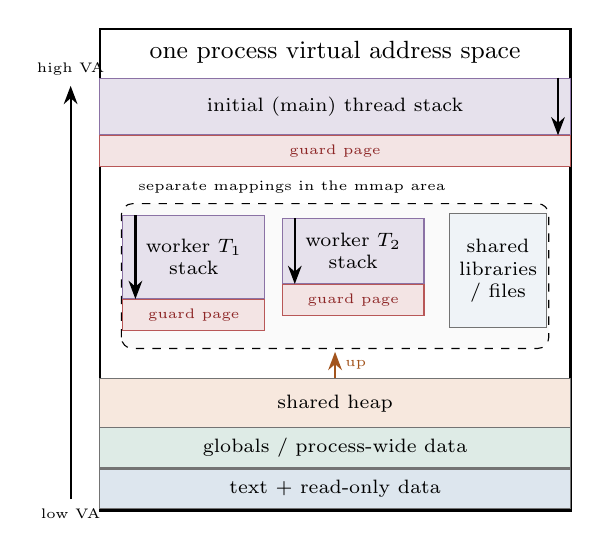
\begin{tikzpicture}[font=\scriptsize,x=.92cm,y=.58cm,
        band/.style={draw=black!55,align=center},
        stack/.style={draw=ospurple!75,fill=ospurple!16,align=center},
        guard/.style={draw=osred!80,fill=osred!13,align=center,
          text=osred!85!black,font=\tiny}]
        % Address-space boundary and direction.
        \draw[thick] (.55,0) rectangle (7.05,10.55);
        \draw[-{Stealth},thick] (.15,.25)--(.15,9.3)
          node[above,font=\tiny]{high VA};
        \node[below,font=\tiny] at (.15,.25) {low VA};

        % Conventional low-address regions.
        \node[band,fill=osblue!15,minimum width=5.98cm,minimum height=.5cm]
          at (3.8,.48) {text + read-only data};
        \node[band,fill=osgreen!15,minimum width=5.98cm,minimum height=.5cm]
          at (3.8,1.38) {globals / process-wide data};
        \node[band,fill=osorange!15,minimum width=5.98cm,minimum height=.62cm]
          (heap) at (3.8,2.35) {shared heap};
        \draw[-{Stealth},thick,osorange!80!black]
          (heap.north)--++(0,.58) node[midway,right,font=\tiny]{up};

        % Worker stacks are separate mappings in the mmap area.
        \draw[dashed,rounded corners,fill=black!2]
          (.85,3.55) rectangle (6.75,6.72);
        \node[anchor=south west,font=\tiny] at (.95,6.74)
          {separate mappings in the mmap area};
        \node[stack,minimum width=1.8cm,minimum height=1.05cm]
          (w1) at (1.85,5.55) {worker $T_1$\\stack};
        \node[guard,minimum width=1.8cm,minimum height=.3cm,
          below=0pt of w1] (g1) {guard page};
        \draw[-{Stealth},thick] ($(w1.north west)+(.18,0)$)--
          ($(w1.south west)+(.18,0)$);
        \node[stack,minimum width=1.8cm,minimum height=.82cm]
          (w2) at (4.05,5.68) {worker $T_2$\\stack};
        \node[guard,minimum width=1.8cm,minimum height=.3cm,
          below=0pt of w2] (g2) {guard page};
        \draw[-{Stealth},thick] ($(w2.north west)+(.18,0)$)--
          ($(w2.south west)+(.18,0)$);
        \node[band,fill=osblue!7,minimum width=1.18cm,minimum height=1.45cm]
          at (6.05,5.25) {shared\\libraries\\/ files};

        % The initial thread also has a thread stack: it is not a separate
        % process-wide stack shared by all threads.
        \node[stack,minimum width=5.98cm,minimum height=.72cm]
          (mainstack) at (3.8,8.85) {initial (main) thread stack};
        \node[guard,minimum width=5.98cm,minimum height=.3cm,
          below=0pt of mainstack] (mainguard) {guard page};
        \draw[-{Stealth},thick] ($(mainstack.north east)+(-.18,0)$)--
          ($(mainstack.south east)+(-.18,0)$);
        \node[anchor=south,font=\small] at (3.8,9.58)
          {one process virtual address space};
      \end{tikzpicture}
    \column{0.32\textwidth}
      \scriptsize
      \begin{itemize}
        \item No separate ``process stack'' exists: the initial thread and every worker each own a stack.
        \item On common downward-growing ABIs, each stack grows toward its lower-address guard page.
        \item Worker stacks are separate mappings whose placement is implementation-dependent.
        \item Reserved stack space need not be fully backed by physical memory.
        \item Exact direction and placement are ABI/OS dependent; this is a common Unix-like convention.
      \end{itemize}
  \end{columns}
\end{frame}

\begin{frame}{Thread control block: the resumable context}
  \begin{center}
    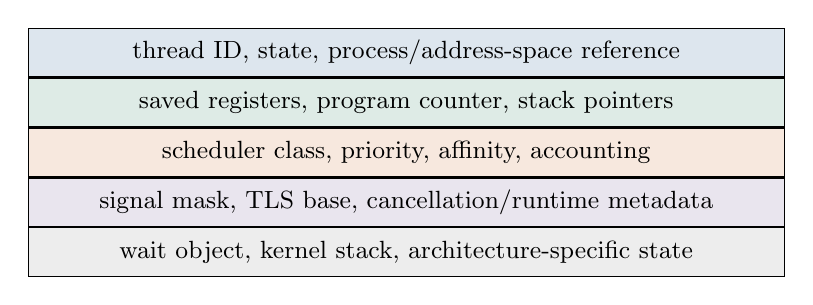
\begin{tikzpicture}[font=\small,node distance=0,
      f/.style={draw,text width=9.2cm,align=center,
        minimum height=.62cm,inner xsep=2mm,anchor=north}]
      \node[f,fill=osblue!15] (id) {thread ID, state, process/address-space reference};
      \node[f,fill=osgreen!15,below=of id] (cpu) {saved registers, program counter, stack pointers};
      \node[f,fill=osorange!15,below=of cpu] (sched) {scheduler class, priority, affinity, accounting};
      \node[f,fill=ospurple!14,below=of sched] (tls) {signal mask, TLS base, cancellation/runtime metadata};
      \node[f,fill=black!7,below=of tls] {wait object, kernel stack, architecture-specific state};
    \end{tikzpicture}
  \end{center}
  \begin{itemize}
    \item Exact fields are OS- and architecture-specific.
    \item Cost may include vector state, TLB effects, cache disruption, and mitigation overhead.
  \end{itemize}
\end{frame}

\begin{frame}{Concurrency is not parallelism}
  \begin{columns}[T,onlytextwidth]
    \column{0.49\textwidth}
      \begin{block}{Concurrency}
        Tasks have overlapping lifetimes and make progress through interleaving, blocking, or asynchronous events.
      \end{block}
      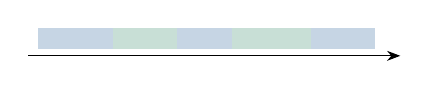
\begin{tikzpicture}[x=.63cm,y=.55cm,font=\scriptsize]
        \draw[-{Stealth}] (0,0)--(7.5,0);
        \fill[osblue!25] (.2,.15) rectangle (1.7,.65);
        \fill[osgreen!25] (1.7,.15) rectangle (3.0,.65);
        \fill[osblue!25] (3.0,.15) rectangle (4.1,.65);
        \fill[osgreen!25] (4.1,.15) rectangle (5.7,.65);
        \fill[osblue!25] (5.7,.15) rectangle (7.0,.65);
      \end{tikzpicture}
    \column{0.47\textwidth}
      \begin{block}{Parallelism}
        Tasks execute at the same instant on distinct processing resources.
      \end{block}
      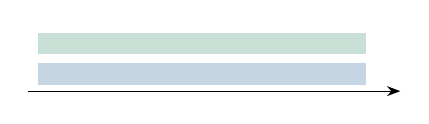
\begin{tikzpicture}[x=.63cm,y=.55cm,font=\scriptsize]
        \draw[-{Stealth}] (0,0)--(7.5,0);
        \fill[osblue!25] (.2,.15) rectangle (6.8,.65) node[midway]{core 0: A};
        \fill[osgreen!25] (.2,.85) rectangle (6.8,1.35) node[midway]{core 1: B};
      \end{tikzpicture}
  \end{columns}
  \smallnote{Asynchrony concerns completion and notification structure; it neither requires nor guarantees another core.}
\end{frame}

\begin{frame}{Why threads---and why not always threads?}
  \small
  \begin{tabularx}{\textwidth}{@{}lXX@{}}
    \toprule
    \textbf{Goal} & \textbf{Potential benefit} & \textbf{New cost/risk} \\
    \midrule
    responsiveness & keep UI/event loop free & coordination and cancellation \\
    overlap CPU and I/O & progress while another task waits & more in-flight state/backpressure \\
    multicore speedup & parallelize independent work & contention and load imbalance \\
    shared state & low-copy communication & races and weak fault isolation \\
    modular servers & one flow per request/task & stack cost and oversubscription \\
    lower creation cost & reuse process resources & no universal fixed speed ratio \\
    \bottomrule
  \end{tabularx}
  \begin{alertblock}{Measure, do not repeat folklore}
    Creation and switching costs depend on mapping, stack policy, cache state, address-space history, mitigations, and workload. Fixed instruction counts or universal multiplicative claims are not portable facts.
  \end{alertblock}
\end{frame}

% =============================================================================
\section{Thread Lifecycle and POSIX Threads}
% =============================================================================

\begin{frame}{Thread lifecycle and resource reclamation}
  \begin{center}
    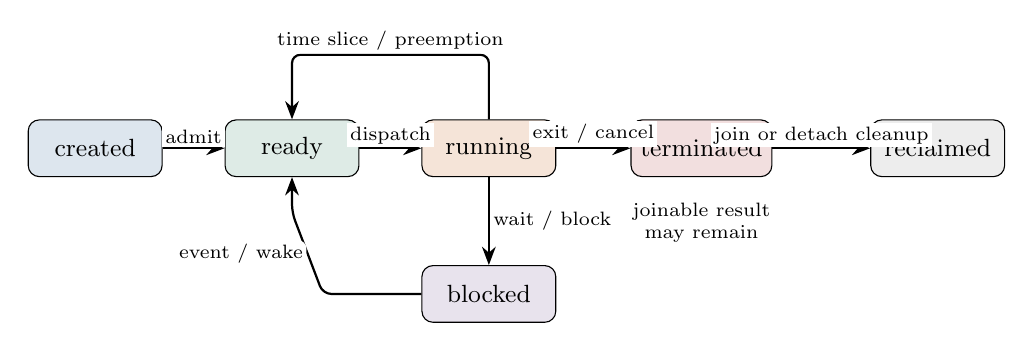
\begin{tikzpicture}[font=\small,
      s/.style={draw,rounded corners,minimum width=1.7cm,minimum height=.72cm},
      a/.style={-{Stealth},thick},
      lab/.style={font=\scriptsize,fill=white,inner sep=1.2pt}]
      \node[s,fill=osblue!15] (new) at (0,1.4) {created};
      \node[s,fill=osgreen!15] (ready) at (2.5,1.4) {ready};
      \node[s,fill=osorange!18] (run) at (5.0,1.4) {running};
      \node[s,fill=ospurple!15] (wait) at (5.0,-.45) {blocked};
      \node[s,fill=osred!15] (term) at (7.7,1.4) {terminated};
      \node[s,fill=black!7] (reap) at (10.7,1.4) {reclaimed};
      \draw[a] (new)--node[lab,above]{admit} (ready);
      \draw[a] (ready)--node[lab,above]{dispatch} (run);
      \coordinate (pre-run) at ($(run.north)+(0,.82)$);
      \coordinate (pre-ready) at ($(ready.north)+(0,.82)$);
      \draw[a,rounded corners=3pt] (run.north)--(pre-run)--
        node[lab,above]{time slice / preemption} (pre-ready)--(ready.north);
      \draw[a] (run.south)--node[lab,right]{wait / block} (wait.north);
      \draw[a,rounded corners=3pt] (wait.west)--++(-1.25,0)--
        node[lab,left]{event / wake} ($(ready.south)+(0,-.45)$)--(ready.south);
      \draw[a] (run)--node[lab,above]{exit / cancel} (term);
      \draw[a] (term)--node[lab,above]{join or detach cleanup} (reap);
      \node[below=2mm of term,font=\scriptsize,align=center]{joinable result\\may remain};
    \end{tikzpicture}
  \end{center}
  \begin{itemize}
    \item A joinable POSIX thread retains join-related resources until joined.
    \item A detached thread releases those resources automatically and cannot be joined.
  \end{itemize}
\end{frame}

\begin{frame}[fragile,shrink=3]{POSIX example I: worker and error contract}
\begin{lstlisting}[language=C]
#include <pthread.h>
#include <stdio.h>
#include <stdlib.h>
#include <string.h>

static void check(int rc, const char *what) {
    if (rc != 0) {
        fprintf(stderr, "%s: %s\n", what, strerror(rc));
        exit(EXIT_FAILURE);
    }
}

static void *worker(void *arg) {
    printf("worker: %s\n", (const char *)arg);
    return (void *)42;       /* demonstration-sized payload */
}
\end{lstlisting}
  \begin{alertblock}{Error contract}
    Most pthread routines return an error number directly. Report it with \code{strerror(rc)}; \code{perror()} reports the unrelated current \code{errno} unless explicitly assigned.
  \end{alertblock}
\end{frame}

\begin{frame}[fragile]{POSIX example II: create, join, and compile}
\begin{lstlisting}[language=C]
int main(void) {
    pthread_t tid; void *result;
    check(pthread_create(&tid, NULL, worker, "hello"), "pthread_create");
    check(pthread_join(tid, &result), "pthread_join");
    printf("result = %ld\n", (long)result);
    return 0;
}
\end{lstlisting}
  \begin{itemize}
    \item Compile with \code{cc -std=c11 -Wall -Wextra -pthread demo.c}.
    \item The argument string remains valid for the worker's lifetime.
    \item Joining both waits for completion and reclaims join-related resources.
  \end{itemize}
\end{frame}

\begin{frame}{Join, detach, and ownership}
  \begin{columns}[T,onlytextwidth]
    \column{0.48\textwidth}
      \begin{block}{Joinable thread}
        \begin{itemize}
          \item another thread calls \code{pthread_join};
          \item join waits for completion and obtains the result;
          \item exactly one successful joiner is expected.
        \end{itemize}
      \end{block}
    \column{0.48\textwidth}
      \begin{block}{Detached thread}
        \begin{itemize}
          \item created detached or later detached;
          \item resources reclaimed at exit;
          \item no later join or result collection.
        \end{itemize}
      \end{block}
  \end{columns}
  \begin{alertblock}{Design rule}
    Every created thread needs a lifetime owner: join it, detach it, or place it under a structured runtime that guarantees cleanup.
  \end{alertblock}
  \note{A terminated-but-unjoined thread is not a Unix zombie process, although it similarly retains some implementation resources.}
\end{frame}

\begin{frame}{Argument and result lifetime hazards}
  \begin{columns}[T,onlytextwidth]
    \column{0.48\textwidth}
      \begin{alertblock}{Unsafe pattern}
        Pass the address of a loop variable or stack object, then change it or leave its scope before the worker reads it.
      \end{alertblock}
    \column{0.48\textwidth}
      \begin{block}{Safe patterns}
        \begin{itemize}
          \item stable per-task objects;
          \item an array alive until all joins;
          \item copied immutable values;
          \item documented result ownership.
        \end{itemize}
      \end{block}
  \end{columns}
  \begin{tcolorbox}[title=Subtlety,colback=osorange!5,colframe=osorange!70]
    Shared addressability does not imply valid lifetime, synchronized access, or ownership. These are separate obligations.
  \end{tcolorbox}
\end{frame}

\begin{frame}{Cancellation should be cooperative}
  \begin{itemize}
    \item Abrupt asynchronous cancellation can leave locks held and invariants broken.
    \item POSIX deferred cancellation acts at cancellation points; cleanup handlers can release resources.
    \item Other runtimes use interruption flags, cancellation tokens, deadlines, or closed channels.
    \item Blocking APIs must participate or be interruptible for timely shutdown.
  \end{itemize}
  \begin{tcolorbox}[title=Structured cancellation,colback=osgreen!5,colframe=osgreen!70]
    Parent scopes should know child tasks, propagate cancellation, and await cleanup before the scope exits.
  \end{tcolorbox}
\end{frame}

\begin{frame}{Signals in a multithreaded process}
  \begin{itemize}
    \item Signal dispositions are generally process-wide; signal masks are per thread.
    \item A process-directed signal may be delivered to one eligible unblocked thread.
    \item A thread-directed signal targets a particular thread.
    \item Synchronous faults arise in the faulting thread, but the default action can terminate the process.
  \end{itemize}
  \begin{block}{Robust pattern}
    Block selected asynchronous signals in workers and dedicate one thread to synchronous receipt with \code{sigwait()}-style APIs.
  \end{block}
\end{frame}

\begin{frame}{Multithreaded \code{fork()}: what the system creates}
  \begin{columns}[T,onlytextwidth]
    \column{0.57\textwidth}
      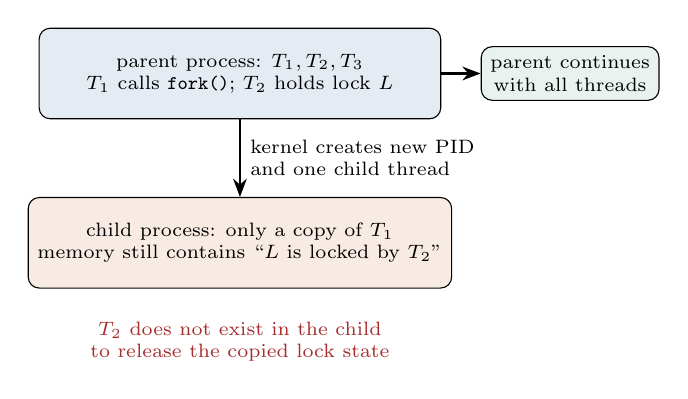
\begin{tikzpicture}[font=\scriptsize,
        p/.style={draw,rounded corners,minimum width=5.1cm,
          minimum height=1.15cm,align=center},
        a/.style={-{Stealth},thick}]
        \node[p,fill=osblue!12] (parent) at (0,2.3)
          {parent process: $T_1,T_2,T_3$\\$T_1$ calls \code{fork()}; $T_2$ holds lock $L$};
        \node[p,fill=osorange!13] (child) at (0,.15)
          {child process: only a copy of $T_1$\\memory still contains ``$L$ is locked by $T_2$''};
        \draw[a] (parent)--node[right,align=left]{kernel creates new PID\\and one child thread} (child);
        \node[draw,fill=osgreen!10,rounded corners,align=center,
          right=5mm of parent] (pres) {parent continues\\with all threads};
        \draw[a] (parent.east)--(pres.west);
        \node[text=osred,align=center,below=3mm of child]
          {$T_2$ does not exist in the child\\to release the copied lock state};
      \end{tikzpicture}
    \column{0.39\textwidth}
      \begin{itemize}
        \item The child receives a new process identity and one execution context: the caller's.
        \item Virtual-memory contents are logically copied, normally using copy-on-write page mappings.
        \item Open descriptors are duplicated and still refer to the same underlying open-file descriptions.
        \item Mutex words and library state are copied as ordinary memory; ownership is not reconstructed.
      \end{itemize}
  \end{columns}
  \note{The exact kernel objects differ by OS. The important abstraction is asymmetric replication: process state is copied, but only the calling thread survives in the child.}
\end{frame}

\begin{frame}{The child-side fork--exec window}
  \begin{center}
    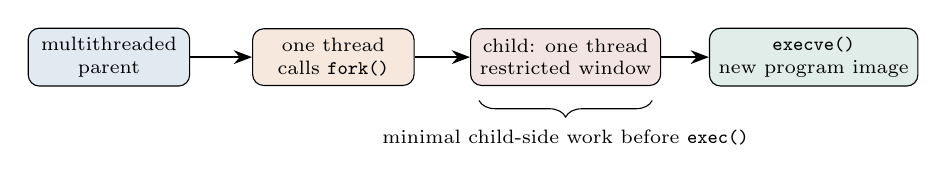
\begin{tikzpicture}[font=\scriptsize,
      s/.style={draw,rounded corners,minimum width=2.05cm,
        minimum height=.72cm,align=center},
      a/.style={-{Stealth},thick}]
      \node[s,fill=osblue!13] (multi) at (0,0) {multithreaded\\parent};
      \node[s,fill=osorange!15] (fork) at (2.85,0) {one thread\\calls \code{fork()}};
      \node[s,fill=osred!13] (window) at (5.8,0)
        {child: one thread\\restricted window};
      \node[s,fill=osgreen!14] (exec) at (8.95,0)
        {\code{execve()}\\new program image};
      \draw[a] (multi)--(fork);
      \draw[a] (fork)--(window);
      \draw[a] (window)--(exec);
      \draw[decorate,decoration={brace,mirror,amplitude=6pt}]
        (4.7,-.55)--(6.9,-.55)
        node[midway,below=7pt,align=center,font=\scriptsize]
          {minimal child-side work before \code{exec()}};
    \end{tikzpicture}
  \end{center}
  \vspace{-1mm}
  \begin{columns}[T,onlytextwidth]
    \column{0.49\textwidth}
      \begin{block}{Preferred paths}\footnotesize
        \begin{itemize}
          \item promptly invoke the new program with \code{exec};
          \item call \code{_exit()} on child-side failure;
          \item prefer \code{posix_spawn()} when it expresses the setup.
        \end{itemize}
      \end{block}
    \column{0.47\textwidth}
      \begin{block}{Role of \code{pthread_atfork()}}\footnotesize
        Prepare, parent, and child handlers can coordinate application-owned locks. They cannot reliably repair hidden locks in arbitrary libraries.
      \end{block}
  \end{columns}
  \begin{tcolorbox}[colback=osred!4,colframe=osred!65]
    \footnotesize Between \code{fork()} and \code{exec()} in the multithreaded child, avoid allocation, buffered I/O, and library code that may acquire copied locks; use only operations permitted in this context.
  \end{tcolorbox}
  \note{A common design is to centralize process spawning or use posix_spawn. At-fork handlers are an escape hatch, not a general reconstruction mechanism for every library's synchronization state.}
\end{frame}

% =============================================================================
\section{User and Kernel Thread Mappings}
% =============================================================================

\begin{frame}{Separate three software layers}
  \begin{center}
    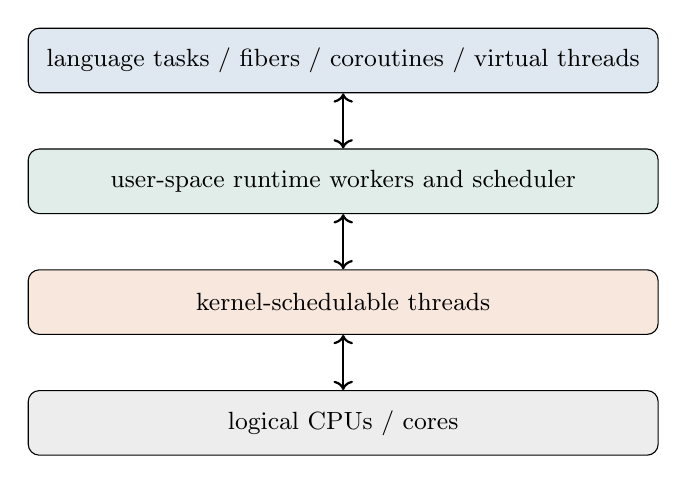
\begin{tikzpicture}[font=\small,node distance=7mm,
      l/.style={draw,rounded corners,minimum width=8cm,minimum height=.82cm},
      a/.style={<->,thick}]
      \node[l,fill=osblue!14] (task) {language tasks / fibers / coroutines / virtual threads};
      \node[l,fill=osgreen!14,below=of task] (runtime) {user-space runtime workers and scheduler};
      \node[l,fill=osorange!16,below=of runtime] (kernel) {kernel-schedulable threads};
      \node[l,fill=black!7,below=of kernel] (cpu) {logical CPUs / cores};
      \draw[a] (task)--(runtime); \draw[a] (runtime)--(kernel); \draw[a] (kernel)--(cpu);
    \end{tikzpicture}
  \end{center}
  \begin{itemize}
    \item User thread may mean an API thread, a runtime task, or a user-managed stack.
    \item The mapping determines visibility, blocking behavior, parallelism, and control.
  \end{itemize}
\end{frame}

\begin{frame}{M:1, 1:1, and M:N at a glance}
  \centering
  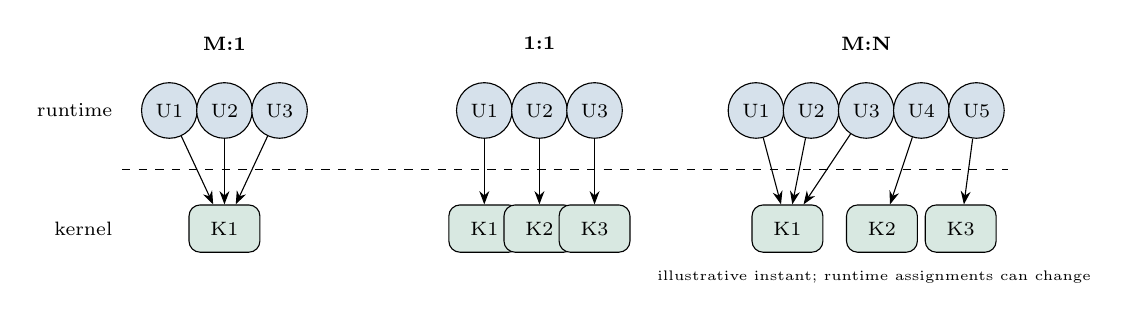
\begin{tikzpicture}[font=\scriptsize,
    u/.style={draw,circle,fill=osblue!18,minimum size=6mm},
    k/.style={draw,rounded corners,fill=osgreen!18,minimum width=9mm,minimum height=6mm},
    a/.style={-{Stealth},thin}]
    \node at (-4,2.35) {\textbf{M:1}};
    \foreach \x/\i in {-4.7/1,-4/2,-3.3/3}{\node[u] (m\i) at (\x,1.5) {U\i};}
    \node[k] (mk) at (-4,0) {K1};
    \foreach \i in {1,2,3}{\draw[a] (m\i)--(mk);}

    \node at (0,2.35) {\textbf{1:1}};
    \foreach \x/\i in {-.7/1,0/2,.7/3}{
      \node[u] (o\i) at (\x,1.5) {U\i};
      \node[k] (ok\i) at (\x,0) {K\i};
      \draw[a] (o\i)--(ok\i);}

    \node at (4.15,2.35) {\textbf{M:N}};
    \foreach \x/\i in {2.75/1,3.45/2,4.15/3,4.85/4,5.55/5}
      {\node[u] (n\i) at (\x,1.5) {U\i};}
    \node[k] (nk1) at (3.15,0) {K1};
    \node[k] (nk2) at (4.35,0) {K2};
    \node[k] (nk3) at (5.35,0) {K3};
    \draw[a] (n1)--(nk1); \draw[a] (n2)--(nk1); \draw[a] (n3)--(nk1);
    \draw[a] (n4)--(nk2); \draw[a] (n5)--(nk3);
    \draw[dashed] (-5.3,.75)--(5.95,.75);
    \node[left] at (-5.3,1.5) {runtime}; \node[left] at (-5.3,0) {kernel};
    \node[font=\tiny,align=center] at (4.25,-.62)
      {illustrative instant; runtime assignments can change};
  \end{tikzpicture}
  \vspace{4mm}
  {\small
  \begin{tabularx}{\textwidth}{@{}lXXX@{}}
    \toprule
    & \textbf{M:1} & \textbf{1:1} & \textbf{M:N} \\
    \midrule
    kernel visibility & one carrier & every API thread & carrier subset \\
    multicore parallelism & at most one & direct & up to $N$ carriers \\
    runtime complexity & low/moderate & low mapping overhead & high \\
    \bottomrule
  \end{tabularx}
  }
\end{frame}

\begin{frame}{Blocking depends on mapping and integration}
  \small
  \begin{tabularx}{\textwidth}{@{}lXXX@{}}
    \toprule
    \textbf{Event} & \textbf{M:1} & \textbf{1:1} & \textbf{M:N runtime} \\
    \midrule
    kernel blocks carrier & all user tasks stop & caller stops & other carriers may run \\
    runtime-aware async I/O & another task can run & another thread runs & carrier can be reused \\
    page fault & sole carrier blocks & faulting thread blocks & other carriers progress \\
    foreign blocking call & blocks unless adapted & blocks caller & may lose/replace carrier \\
    \bottomrule
  \end{tabularx}
  \begin{alertblock}{Correction to the textbook slogan}
    A blocking call stops the whole process only for a pure M:1 runtime using an unadapted blocking operation, not for every user-managed threading system.
  \end{alertblock}
\end{frame}

\begin{frame}{One-to-one: direct OS integration}
  \begin{itemize}
    \item Each application thread corresponds to a kernel-schedulable thread.
    \item Blocking, priorities, affinity, signals, and profiling integrate directly with the OS.
    \item Different threads from one process can execute simultaneously.
    \item Each consumes kernel metadata and stack/address-space resources; enormous counts are costly.
  \end{itemize}
  \begin{tcolorbox}[title=Common deployment,colback=osgreen!5,colframe=osgreen!70]
    Native POSIX threads on Linux and platform threads on mainstream desktop/server systems typically expose 1:1 behavior.
  \end{tcolorbox}
\end{frame}

\begin{frame}{Many-to-many: runtime scheduling over carriers}
  \begin{itemize}
    \item Many logical tasks are multiplexed over a bounded or elastic carrier set.
    \item Runtime can use lightweight stacks, task-aware blocking, local queues, and work stealing.
    \item Parallelism is bounded by carriers and CPU capacity, not logical task count.
    \item Native calls, TLS assumptions, pinning, debugging, and profiling add complexity.
  \end{itemize}
  \begin{alertblock}{Logical task count is not CPU speed}
    A million lightweight tasks may improve throughput for blocked workloads, but cannot make fixed CPU work exceed core capacity or algorithmic parallelism.
  \end{alertblock}
\end{frame}

\begin{frame}{Modern examples: goroutines and virtual threads}
  \small
  \begin{itemize}
    \item Go multiplexes goroutines over OS threads, and its runtime can preempt goroutines; programs must not assume a schedule order.
    \item Java virtual threads are user-mode \code{Thread} instances scheduled over carrier platform threads.
    \item Virtual threads target high-throughput workloads with abundant blocking, especially I/O; they are not faster CPU threads.
    \item Both retain a thread-like blocking style while moving multiplexing into the language runtime.
  \end{itemize}
  \begin{tcolorbox}[title=Abstraction benefit,colback=osblue!4,colframe=osblue!65]
    Runtime-aware tasks can make blocking source code scale like event-driven code when blocking can release or unmount the carrier.
  \end{tcolorbox}
  \smallnote{Source basis: Go documentation and OpenJDK JEP 444 / Java virtual-thread documentation, accessed August 2026.}
\end{frame}

\begin{frame}{Stackful threads versus stackless async tasks}
  \small
  \begin{tabularx}{\textwidth}{@{}lXX@{}}
    \toprule
    & \textbf{Stackful thread/fiber} & \textbf{Stackless async state machine} \\
    \midrule
    suspension & almost anywhere runtime permits & explicit \code{await}/yield points \\
    state & preserved call stack & compiler-generated state object \\
    coding style & direct sequential flow & async propagation/function coloring \\
    memory & stack or segmented stack & task object and captured state \\
    migration & runtime-dependent & executor-dependent \\
    debugging & familiar stack per task & logical async stacks needed \\
    \bottomrule
  \end{tabularx}
  \smallnote{Coroutines describe suspend/resume control flow; M:1 versus M:N depends on the executor and runtime.}
\end{frame}

% =============================================================================
\section{Pools, Scheduling, and Scalability}
% =============================================================================

\begin{frame}{Thread-per-task versus a worker pool}
  \begin{columns}[T,onlytextwidth]
    \column{0.48\textwidth}
      \begin{block}{Thread per task}
        \begin{itemize}
          \item simple ownership and blocking style;
          \item natural stack isolation;
          \item native threads cost resources at high concurrency.
        \end{itemize}
      \end{block}
    \column{0.48\textwidth}
      \begin{block}{Pool of workers}
        \begin{itemize}
          \item amortizes creation and bounds workers;
          \item requires queues and backpressure;
          \item blocking tasks can exhaust the pool.
        \end{itemize}
      \end{block}
  \end{columns}
  \begin{alertblock}{Queueing is part of the API contract}
    An unbounded queue converts overload into latency and memory growth. A bounded queue requires rejection, shedding, or producer backpressure.
  \end{alertblock}
\end{frame}

\begin{frame}{Work stealing balances irregular parallelism}
  \begin{center}
    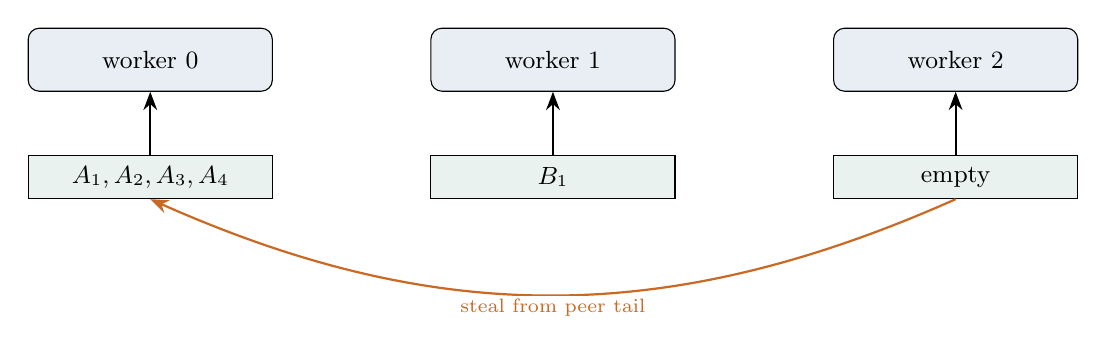
\begin{tikzpicture}[font=\small,node distance=8mm,
      w/.style={draw,rounded corners,minimum width=3.1cm,minimum height=.8cm,fill=osblue!10},
      q/.style={draw,minimum width=3.1cm,minimum height=.55cm,fill=osgreen!10}]
      \node[w] (w0) {worker 0}; \node[q,below=of w0] (q0) {$A_1,A_2,A_3,A_4$};
      \node[w,right=2cm of w0] (w1) {worker 1}; \node[q,below=of w1] (q1) {$B_1$};
      \node[w,right=2cm of w1] (w2) {worker 2}; \node[q,below=of w2] (q2) {empty};
      \draw[-{Stealth},thick,osorange] (q2.south) to[bend left=24]
        node[below,font=\scriptsize,fill=white,inner sep=1pt]{steal from peer tail} (q0.south);
      \draw[-{Stealth},thick] (q0)--(w0);
      \draw[-{Stealth},thick] (q1)--(w1);
      \draw[-{Stealth},thick] (q2)--(w2);
    \end{tikzpicture}
  \end{center}
  \begin{itemize}
    \item Workers prefer local queues for locality and low contention.
    \item Idle workers steal tasks, improving balance for recursive or irregular work.
    \item Blocking, priorities, affinity, and non-stealable tasks complicate the ideal.
  \end{itemize}
\end{frame}

\begin{frame}{Oversubscription: runnable threads exceed CPUs}
  If $R$ runnable CPU-bound threads compete for $P$ logical CPUs:
  \begin{itemize}
    \item $R\le P$ can underutilize CPUs if tasks block or are imbalanced;
    \item $R\gg P$ increases preemption, cache/TLB churn, contention, and tail latency;
    \item modest oversubscription can hide blocking but must be workload-driven;
    \item simultaneous multithreading does not make each logical CPU a full core.
  \end{itemize}
  \begin{tcolorbox}[title=Sizing principle,colback=osgreen!5,colframe=osgreen!70]
    Tie CPU-bound pools to measured CPU capacity. Give blocking pools explicit concurrency and backpressure limits instead of arbitrary huge sizes.
  \end{tcolorbox}
\end{frame}

\begin{frame}{Amdahl's law bounds ideal speedup}
  If fraction $p$ is perfectly parallel and $1-p$ remains serial,
  \[
    S(N)=\frac{1}{(1-p)+p/N}.
  \]
  For $p=0.95$ and $N=16$:
  \[
    S(16)=\frac{1}{0.05+0.95/16}\approx 9.14,
  \]
  not $16\times$.
  \begin{itemize}
    \item Synchronization, communication, imbalance, and memory bandwidth reduce speedup further.
    \item Increasing problem size can change $p$; weak scaling asks a different question.
  \end{itemize}
  \note{Ask why threads can slow a high-$p$ program: scheduling cost, coherence, shared bottlenecks, NUMA, and critical sections are outside the ideal equation.}
\end{frame}

\begin{frame}{Little's law connects concurrency and throughput}
  For a stable system,
  \[
    L=\lambda W,
  \]
  where $L$ is average in-flight work, $\lambda$ throughput, and $W$ average response time.
  \begin{exampleblock}{Example}
    At $\lambda=2{,}000$ requests/s and $W=50$ ms, average concurrency is
    $L=2000\times0.05=100$ requests.
  \end{exampleblock}
  \begin{alertblock}{Capacity lesson}
    More threads do not create capacity. If arrivals exceed service capacity, queues and latency grow; bound concurrency and apply backpressure.
  \end{alertblock}
\end{frame}

% =============================================================================
\section{Memory Semantics and Performance Hazards}
% =============================================================================

\begin{frame}{A data race is more than unlucky interleaving}
  Conflicting accesses race when concurrent, at least one is a write, and no synchronization orders them.
  \begin{columns}[T,onlytextwidth]
    \column{0.48\textwidth}
      \begin{alertblock}{Naive increment}
        \code{x++} is read--modify--write. Two threads can read one old value and lose an update.
      \end{alertblock}
    \column{0.48\textwidth}
      \begin{block}{Language consequence}
        In C/C++, a race on a non-atomic object is undefined behavior, allowing compiler transformations beyond a lost update.
      \end{block}
  \end{columns}
  \smallnote{Correctness requires atomicity and a defined memory-order relationship for visibility.}
\end{frame}

\begin{frame}[fragile]{Atomic counter versus protected invariant}
\begin{lstlisting}[language=C]
#include <stdatomic.h>

static _Atomic unsigned long requests = 0;

void count_request(void) {
    atomic_fetch_add_explicit(&requests, 1, memory_order_relaxed);
}
\end{lstlisting}
  \begin{itemize}
    \item Relaxed atomicity suits an independent statistics counter when it publishes no other data.
    \item A mutex is clearer for multi-field invariants such as balance plus transaction log.
    \item Lock-free does not imply faster, fair, wait-free, or free of cache contention.
  \end{itemize}
\end{frame}

\begin{frame}{Happens-before: the visibility contract}
  Synchronization creates ordering edges constraining compiler and hardware reordering.
  \begin{center}
    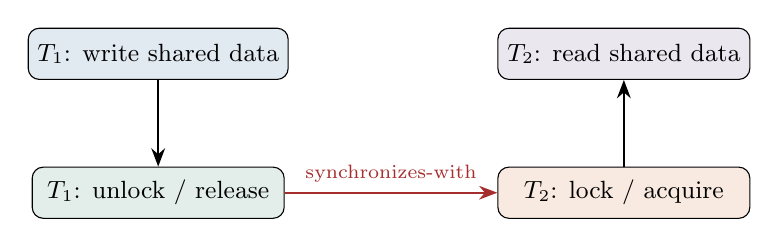
\begin{tikzpicture}[font=\small,node distance=1.1cm,
      e/.style={draw,rounded corners,minimum width=3.2cm,minimum height=.65cm},
      a/.style={-{Stealth},thick}]
      \node[e,fill=osblue!13] (w) {$T_1$: write shared data};
      \node[e,fill=osgreen!13,below=of w] (unlock) {$T_1$: unlock / release};
      \node[e,fill=osorange!14,right=2.7cm of unlock] (lock) {$T_2$: lock / acquire};
      \node[e,fill=ospurple!13,above=of lock] (r) {$T_2$: read shared data};
      \draw[a] (w)--(unlock);
      \draw[a,osred] (unlock.east)--
        node[midway,above=2pt,font=\scriptsize,fill=white,inner sep=1.5pt]
          {synchronizes-with}
        (lock.west);
      \draw[a] (lock)--(r);
    \end{tikzpicture}
  \end{center}
  By transitivity, the write happens-before the read, so the synchronized reader observes a state allowed by the language memory model.
\end{frame}

\begin{frame}{False sharing: independent data, shared cache line}
  \begin{center}
    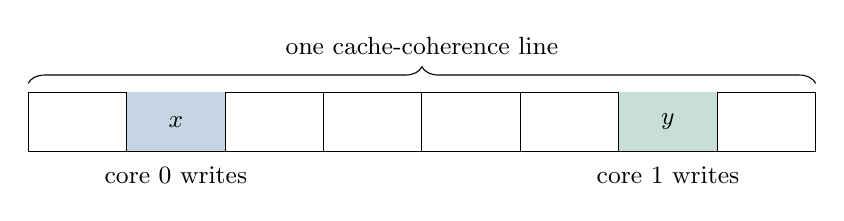
\begin{tikzpicture}[font=\small,x=1.25cm,y=.75cm]
      \foreach \i in {0,...,7}{\draw (\i,0) rectangle (\i+1,1);}
      \fill[osblue!25] (1,0) rectangle (2,1); \node at (1.5,.5) {$x$};
      \fill[osgreen!25] (6,0) rectangle (7,1); \node at (6.5,.5) {$y$};
      \draw[decorate,decoration={brace,amplitude=6pt}] (0,1.15)--(8,1.15)
        node[midway,above=7pt]{one cache-coherence line};
      \node[below] at (1.5,-.1) {core 0 writes};
      \node[below] at (6.5,-.1) {core 1 writes};
    \end{tikzpicture}
  \end{center}
  \begin{itemize}
    \item $x$ and $y$ need not be logically shared, yet writes invalidate the full line.
    \item Symptoms include poor scaling and coherence traffic without a lock hotspot.
    \item Padding/alignment can help but changes layout and wastes cache capacity.
  \end{itemize}
\end{frame}

\begin{frame}{Thread-local storage is isolation, not synchronization}
  \begin{itemize}
    \item TLS gives each thread a distinct instance of a named object.

    \item Useful for per-thread caches, random state, error state, and scratch buffers.
    \item TLS reduces sharing but can increase footprint and complicate aggregation.
    \item Logical tasks multiplexed over workers must not confuse carrier TLS with task-local state.
  \end{itemize}
  \begin{alertblock}{Runtime distinction}
    Thread-local, fiber-local, task-local, and request-context storage have different lifetimes and migration behavior.
  \end{alertblock}
\end{frame}

\begin{frame}{Fault isolation and failure containment}
  \small
  \begin{tabularx}{\textwidth}{@{}lXX@{}}
    \toprule
    & \textbf{Separate processes} & \textbf{Threads in one process} \\
    \midrule
    address isolation & hardware-enforced by default & shared; pointer bugs cross components \\
    communication & IPC/serialization/shared maps & direct loads/stores \\
    crash scope & often one process/service & often whole process \\
    resource control & process/cgroup controls & shared limits, per-thread CPU policy \\
    deployment & heavier, independently restartable & lightweight composition \\
    \bottomrule
  \end{tabularx}
  \begin{tcolorbox}[title=Architecture principle,colback=osorange!5,colframe=osorange!70]
    Choose process boundaries for trust and failure containment; choose threads/tasks for efficient cooperation inside a trust boundary.
  \end{tcolorbox}
\end{frame}

% =============================================================================
\section{Design, Debugging, and Observation}
% =============================================================================

\begin{frame}{Choosing an execution model}
  \small
  \begin{tabularx}{\textwidth}{@{}lXX@{}}
    \toprule
    \textbf{Workload} & \textbf{Good starting point} & \textbf{Primary concern} \\
    \midrule
    CPU-parallel numerical kernel & bounded native worker pool & locality and bandwidth \\
    many blocked network requests & async or lightweight M:N tasks & backpressure and pinning \\
    GUI application & event thread + bounded workers & never block UI dispatcher \\
    untrusted plugins/services & process isolation + IPC & containment and permissions \\
    recursive irregular tasks & work-stealing pool & granularity and stealing cost \\
    real-time control & bounded native threads & WCET, locks, priorities \\
    \bottomrule
  \end{tabularx}
\end{frame}

\begin{frame}{Debugging nondeterministic failures}
  \begin{itemize}
    \item Reproduce under varied CPU counts, affinity, timing, and optimization.
    \item Use race detectors/sanitizers for unsynchronized memory access.
    \item Record lock order, blocking duration, queue length, and ownership.
    \item Prefer deterministic tests for concurrent components where possible.
    \item Capture thread dumps and scheduler traces during stalls.
    \item Distinguish deadlock, livelock, starvation, inversion, and overload.
  \end{itemize}
  \begin{alertblock}{Heisenbug warning}
    Logging and debugging alter timing and layout. No failure under a debugger is not evidence of correctness.
  \end{alertblock}
\end{frame}

\begin{frame}[fragile]{Observing threads on Linux}
\begin{lstlisting}[language=bash]
# List kernel-visible threads in one process
ps -L -p "$PID" -o pid,tid,psr,stat,pri,ni,pcpu,comm

# Per-thread procfs entries and interactive view
ls /proc/$PID/task
cat /proc/$PID/task/$TID/status
top -H -p "$PID"

# Trace creation, waiting, and termination
strace -f -e clone,clone3,futex,exit ./program
\end{lstlisting}
  \smallnote{An M:N runtime may expose only carrier OS threads here; use runtime-specific diagnostics for logical tasks.}
\end{frame}

\begin{frame}{Code-review checklist for thread creation}
  \begin{enumerate}
    \item Who owns the task and how is it stopped?
    \item Is its argument valid until consumed?
    \item Is every joinable thread joined exactly once, or detached?
    \item What bounds active and queued work?
    \item What synchronization establishes happens-before?
    \item Can blocking exhaust a pool or pin a carrier?
    \item What happens on partial startup failure?
    \item Are errors, cancellation, and results propagated?
  \end{enumerate}
\end{frame}

% =============================================================================
\section{Synthesis}
% =============================================================================

\begin{frame}{Misconceptions corrected}
  \scriptsize
  \begin{tabularx}{\textwidth}{@{}XcX@{}}
    \toprule
    \textbf{Misconception} & & \textbf{Precise statement} \\
    \midrule
    Process is always the CPU scheduling unit. & $\Rightarrow$ & Mainstream kernels normally dispatch threads/tasks. \\
    User threads cannot run in parallel. & $\Rightarrow$ & M:1 cannot; M:N can use multiple carriers. \\
    Any blocking call blocks every user thread. & $\Rightarrow$ & It depends on mapping and runtime-aware I/O. \\
    Threads are always much faster than processes. & $\Rightarrow$ & Cost depends on implementation and workload state. \\
    \code{volatile} fixes races. & $\Rightarrow$ & Use language-defined atomics or synchronization. \\
    More threads produce more CPU throughput. & $\Rightarrow$ & Cores, serial work, and bottlenecks bound speedup. \\
    Virtual threads make CPU code faster. & $\Rightarrow$ & They primarily scale blocked concurrency. \\
    Different variables cannot contend. & $\Rightarrow$ & False sharing couples writes in one cache line. \\
    \bottomrule
  \end{tabularx}
\end{frame}

\begin{frame}{Key takeaways}
  \begin{itemize}
    \item A process is a protection/resource container; a thread is an execution context.
    \item Shared addressing lowers communication cost and fault isolation.
    \item M:1, 1:1, and M:N determine visibility, blocking, and parallelism.
    \item Correct lifecycle management needs explicit ownership, join/detach, and cancellation.
    \item Pools and lightweight tasks require bounded queues and backpressure.
    \item Amdahl's law, balance, and memory bandwidth limit speedup.
    \item Synchronization defines atomicity and visibility; false sharing can dominate cost.
    \item Runtime multiplexing cannot evade finite CPU capacity.
  \end{itemize}
\end{frame}

\begin{frame}{Next week: synchronization and memory ordering}
  \begin{itemize}
    \item critical-section safety and liveness requirements;
    \item mutexes, semaphores, condition variables, and monitors;
    \item atomic read--modify--write instructions;
    \item acquire/release and sequential consistency;
    \item deadlock conditions, avoidance, and lock ordering;
    \item bounded-buffer and readers--writers problems;
    \item lock-free versus wait-free progress.
  \end{itemize}
  \begin{tcolorbox}[title=Preparation,colback=osgreen!5,colframe=osgreen!70]
    Review invariants, interleavings, cache coherence, and the difference between atomicity and visibility.
  \end{tcolorbox}
\end{frame}

% =============================================================================
\appendix
\section{Appendix: Code and Exploration}
% =============================================================================

\begin{frame}{Knowledge check: execution state}
  \begin{enumerate}
    \item Which resources are process-wide and which are per-thread?
    \item Why does each thread require a separate stack?
    \item Can a single-threaded process run on two cores simultaneously?
    \item Distinguish concurrency, parallelism, and asynchrony.
    \item Why can one thread's invalid pointer terminate all threads?
    \item How can TLS fail for tasks that migrate carriers?
  \end{enumerate}
\end{frame}

\begin{frame}{Exercise: repair a pthread program}
  A loop creates eight threads and passes \code{\&i} as each argument. The loop ends before joins, failures call \code{perror()}, and some successful threads are never joined.
  \begin{enumerate}
    \item Identify the lifetime and data-race problem.
    \item Replace it with stable per-thread argument storage.
    \item Correct error reporting using returned error codes.
    \item Handle partial creation failure without leaks.
    \item Define result ownership and cleanup.
    \item Compile with warnings and run a thread sanitizer.
  \end{enumerate}
\end{frame}

\begin{frame}{Exercise: choose a mapping and pool size}
  Compare three services:
  \begin{enumerate}
    \item 32 CPU-heavy image transforms on a 16-core server;
    \item 100,000 mostly blocked network connections;
    \item 20 untrusted plugins processing customer documents.
  \end{enumerate}
  For each:
  \begin{itemize}
    \item choose processes, 1:1 threads, M:N tasks, or an event loop;
    \item bound active and queued work;
    \item identify the bottleneck and failure boundary;
    \item state what evidence would change the design.
  \end{itemize}
\end{frame}

\begin{frame}{Exercise: Amdahl and overhead}
  A program is 92\% parallel. Each parallel worker adds 0.3\% of original runtime in scheduling and communication overhead.
  \begin{enumerate}
    \item Compute ideal speedup for $N=2,4,8,16,32$.
    \item Add overhead $0.003N$ to the normalized denominator.
    \item Which $N$ gives the best modeled speedup?
    \item Why might memory bandwidth make performance peak earlier?
    \item Distinguish strong scaling from weak scaling.
  \end{enumerate}
\end{frame}

\begin{frame}{Exercise: diagnose a scalability collapse}
  A counter benchmark scales to four cores, then slows sharply. No mutex appears; each worker updates a distinct array element.
  \begin{enumerate}
    \item Draw a plausible false-sharing layout.
    \item What profiling evidence would support the diagnosis?
    \item Compare padding, sharding, and batched aggregation.
    \item Explain padding's memory-footprint trade-off.
    \item Why might relaxed atomics not fix performance?
  \end{enumerate}
\end{frame}

\subsection{Code examples}

\begin{frame}[fragile]{Code example: parallel sum worker}
\begin{lstlisting}[language=C]
#include <pthread.h>
#include <stdio.h>
#include <stdlib.h>
#include <string.h>
enum { N = 4 };
struct job { const int *x; size_t lo, hi; long sum; };
static void *sum_part(void *p) {
    struct job *j = p;
    j->sum = 0;
    for (size_t i = j->lo; i < j->hi; ++i) j->sum += j->x[i];
    return NULL;
}
\end{lstlisting}
  \begin{itemize}
    \item Each worker reads the shared input and writes only its own \code{job} record.
    \item The driver shown next supplies non-overlapping ranges and joins before reducing results.
  \end{itemize}
  \smallnote{Combine with the next slide; compile using \code{cc -std=c11 -Wall -Wextra -pthread sum.c}. Expected output: \code{sum = 78}.}
  \note{The disjoint writes avoid a mutex for this example. The join operation also orders worker completion before the main thread reads each partial sum.}
\end{frame}

\begin{frame}[fragile]{Code example: create, join, and reduce}
\begin{lstlisting}[language=C,aboveskip=0pt,belowskip=0pt]
int main(void) {
    static const int x[12] = {1,2,3,4,5,6,7,8,9,10,11,12};
    pthread_t t[N]; struct job j[N]; size_t made = 0;
    for (size_t i = 0; i < N; ++i) {
        j[i] = (struct job){x, 3*i, 3*(i+1), 0};
        int e = pthread_create(&t[i], NULL, sum_part, &j[i]);
        if (e) {
            fprintf(stderr, "create: %s\n", strerror(e));
            while (made) pthread_join(t[--made], NULL);
            return EXIT_FAILURE;
        }
        ++made;
    }
    long total = 0;
    for (size_t i = 0; i < N; ++i) {
        int e = pthread_join(t[i], NULL);
        if (e) { fprintf(stderr, "join: %s\n", strerror(e)); return EXIT_FAILURE; }
        total += j[i].sum;
    }
    printf("sum = %ld\n", total);
    return EXIT_SUCCESS;
}
\end{lstlisting}
\note{Combine this main function with the worker slide above and compile using cc -std=c11 -Wall -Wextra -pthread. The output is sum = 78. The fixed partition keeps the example focused on ownership and joining; production code should derive ranges from input length and account for load imbalance. On partial startup failure, already-created joinable threads are joined before return.}
\end{frame}

\begin{frame}[fragile]{Code example: constrained fork--exec--wait}
\begin{lstlisting}[language=C]
#include <errno.h>
#include <stdio.h>
#include <stdlib.h>
#include <sys/wait.h>
#include <unistd.h>
extern char **environ;
int main(void) {
    pid_t child = fork();
    if (child < 0) { perror("fork"); return EXIT_FAILURE; }
    if (child == 0) {
        char *const argv[] = {"/usr/bin/printf", "child ran\n", NULL};
        execve(argv[0], argv, environ);
        _exit(127);
    }
    int status;
    pid_t r;
    do { r = waitpid(child, &status, 0); } while (r == -1 && errno == EINTR);
    if (r == -1) { perror("waitpid"); return EXIT_FAILURE; }
    if (WIFEXITED(status)) printf("exit: %d\n", WEXITSTATUS(status));
    return EXIT_SUCCESS;
}
\end{lstlisting}
\note{Linux-oriented example; adjust the executable path elsewhere. Compile with cc -std=c11 -Wall -Wextra. This uses execve with an explicit path and inherited environment. In a multithreaded child, keep the fork-to-exec path minimal and use only permitted operations. _exit avoids flushing copied stdio buffers or invoking inherited atexit handlers. waitpid retries only when interrupted.}
\end{frame}

\subsection{Exploratory topics}

\begin{frame}{Exploration: runtimes and execution semantics}
  \begin{itemize}
    \item \textbf{POSIX lifecycle:} attributes, cancellation points, signal masks, cleanup handlers, and at-fork handlers;
    \item \textbf{Memory models:} compare C/C++ atomics and Java happens-before guarantees;
    \item \textbf{Task runtimes:} work stealing, fork--join decomposition, structured concurrency, and task-local state;
    \item \textbf{Go:} inspect goroutine scheduling, blocking system calls, and runtime trace output;
    \item \textbf{Java:} examine virtual-thread carrier scheduling, pinning conditions, and observability tools;
    \item \textbf{Rust:} compare async executors, task migration, ownership, and \code{Send} constraints.
  \end{itemize}
  \begin{tcolorbox}[title=Mini-investigation,colback=osorange!5,colframe=osorange!70]
    Choose one runtime. Trace a blocking operation and explain whether it blocks a kernel thread, a carrier, a logical task, or the whole process.
  \end{tcolorbox}
\end{frame}

\begin{frame}{Exploration: scalability, locality, and testing}
  \small
  \begin{itemize}
    \item \textbf{Memory hierarchy:} measure false sharing, cache coherence traffic, and NUMA placement effects;
    \item \textbf{Scheduling:} compare work stealing with static partitioning under balanced and skewed workloads;
    \item \textbf{Correctness tools:} compare race detectors, thread sanitizers, and model checking;
    \item \textbf{Reproducibility:} design deterministic tests for cancellation, shutdown, and partial startup failure;
    \item \textbf{Fault boundaries:} compare thread pools with worker processes for untrusted or crash-prone tasks;
    \item \textbf{Performance study:} report throughput and latency percentiles while sweeping worker count and queue capacity.
  \end{itemize}
  \begin{tcolorbox}[title=Suggested project,colback=osgreen!5,colframe=osgreen!70]
    Build a bounded task executor. Document its ownership model, queue policy, shutdown behavior, and measurements under CPU-heavy, blocking, and imbalanced workloads.
  \end{tcolorbox}
\end{frame}

\subsection{Debugging exercises: deliberate faults}

\begin{frame}[fragile]{Exercise: a shared counter that loses updates}
  \scriptsize
\begin{lstlisting}[language=C]
volatile long total = 0;
static void *worker(void *unused) {
    (void)unused;
    for (int i = 0; i < 100000; ++i)
        ++total;
    return NULL;
}
\end{lstlisting}
  \begin{enumerate}
    \item Start two workers and join both. Is the final value guaranteed to be 200000?
    \item Identify the language-level fault and explain why \code{volatile} does not establish thread synchronization.
    \item Predict how a race detector will characterize this access.
  \end{enumerate}
  \begin{tcolorbox}[title=Hint,colback=osorange!5,colframe=osorange!70]
    Expand \code{++total} into its conceptual read, modify, and write steps; consider two workers interleaving those steps.
  \end{tcolorbox}
\end{frame}

\begin{frame}[fragile]{Exercise: thread arguments with the wrong lifetime}
  \scriptsize
\begin{lstlisting}[language=C]
static void *print_id(void *p) {
    int id = *(int *)p;
    printf("worker %d\\n", id);
    return NULL;
}
int main(void) {
    pthread_t t[8];
    for (int i = 0; i < 8; ++i)
        pthread_create(&t[i], NULL, print_id, &i);
    for (int i = 0; i < 8; ++i) pthread_join(t[i], NULL);
}
\end{lstlisting}
  \begin{enumerate}
    \item List the different outputs that might appear, and explain why output order is not the only problem.
    \item Identify the lifetime and concurrent-access hazards.
    \item Propose a test or instrumentation that could make the bug easier to observe.
  \end{enumerate}
  \begin{tcolorbox}[title=Hint,colback=osorange!5,colframe=osorange!70]
    Track exactly which object each worker receives, how long that object lives, and whether the loop can change it before a worker reads it.
  \end{tcolorbox}
\end{frame}

\begin{frame}[fragile]{Exercise: inconsistent lock ordering}
  \scriptsize
\begin{lstlisting}[language=C]
pthread_mutex_t a = PTHREAD_MUTEX_INITIALIZER;
pthread_mutex_t b = PTHREAD_MUTEX_INITIALIZER;
/* Worker A */
pthread_mutex_lock(&a); pthread_mutex_lock(&b);
/* critical section */
pthread_mutex_unlock(&b); pthread_mutex_unlock(&a);
/* Worker B performs the same work with reverse acquisition order. */
pthread_mutex_lock(&b); pthread_mutex_lock(&a);
/* critical section */
pthread_mutex_unlock(&a); pthread_mutex_unlock(&b);
\end{lstlisting}
  \begin{enumerate}
    \item Give an interleaving in which both workers stop making progress.
    \item Draw the wait-for/resource-allocation graph and identify the cycle.
    \item Describe a design invariant that would prevent this class of failure; do not rely on timing.
  \end{enumerate}
  \begin{tcolorbox}[title=Hint,colback=osorange!5,colframe=osorange!70]
    Assume each worker acquires its first mutex before the other worker attempts its second. Who owns each lock, and what is each waiting for?
  \end{tcolorbox}
\end{frame}

\begin{frame}[fragile]{Exercise: condition-variable predicate bug}
  \scriptsize
\begin{lstlisting}[language=C]
/* mutex is held on entry; count is the number of queued items */
static void consume_one(void) {
    if (count == 0)
        pthread_cond_wait(&ready, &mutex);
    --count;                 /* claim one item */
    pthread_mutex_unlock(&mutex);
}
/* Producer adds one item while holding mutex, then: */
pthread_cond_broadcast(&ready);
\end{lstlisting}
  \begin{enumerate}
    \item With two consumers waiting and one item added, describe a legal execution that breaks the queue invariant.
    \item Explain what the condition-variable notification does—and what it does not promise.
    \item Identify another wakeup case the consumer must be prepared to handle.
  \end{enumerate}
  \begin{tcolorbox}[title=Hint,colback=osorange!5,colframe=osorange!70]
    Treat the shared predicate as the truth; a wakeup is only a reason to re-check it. Consider both competing consumers and spurious wakeups.
  \end{tcolorbox}
\end{frame}

\end{document}

